\documentclass[10pt,a4paper,twocolumn]{article}

% --- Packages ---
\usepackage[utf8]{inputenc}
\usepackage[T1]{fontenc}
\usepackage[margin=0.75in]{geometry}
\usepackage{booktabs}
\usepackage{hyperref}
\usepackage[round]{natbib}
\usepackage{amsmath}
\usepackage{amssymb}
\usepackage{graphicx}
\usepackage{xspace}
\usepackage{enumitem}
\usepackage{adjustbox}
\usepackage{dblfloatfix}   % fix placement of wide floats in twocolumn

\hypersetup{
  colorlinks=true,
  linkcolor=blue,
  citecolor=blue,
  urlcolor=blue
}

\title{Which Context Surface Do LLMs Respect Most\\for Org-Specific Knowledge?\\[0.5em]
\large An Evaluation Framework Using Controlled Retrieval Variants}

\author{Srinivas Vaddi\\Independent Researcher}

\date{March 2026}

\begin{document}

\maketitle
\begin{abstract}
Large language models handle public coding benchmarks well, but struggle with org-specific conventions --- internal logging formats, prescribed API calls, compliance patterns --- that never appear in training data. When a code repair task requires both fixing a bug \emph{and} following an org policy, models must retrieve the relevant information somehow.
The question is: which delivery mechanism actually works?

This paper introduces \textbf{Script30}, a pilot benchmark designed to
answer that question empirically. Seven context surfaces are evaluated --- from no context at all to autonomous retrieval with \texttt{AGENTS.md} and \texttt{SKILL.md} --- across two
model families (\texttt{claude-haiku-4-5} and \texttt{gpt-5.1-codex-mini}, $n{=}3$ each, 1,229 scored runs).
The results are model-dependent. Haiku peaked with \texttt{SKILL.md} plus retrieval tools (\textbf{69.2\%}), well above oracle injection (\textbf{65.4\%}) and the no-guide agentic
baseline (\textbf{39.7\%}). For Codex, static injection (\textbf{43.0\%}) significantly outperformed tool-based retrieval (\textbf{20.0\%}), suggesting oracle injection is the more effective surface for this model family.

These are directional findings from a small pilot. The benchmark, harness, and all run artefacts are at \url{https://github.com/vaddisrinivas/moltsnip} (branch \texttt{arxiv-v1}).
\end{abstract}

% ===================================================================
\section{Introduction}
\label{sec:introduction}

Public benchmarks such as HumanEval~\citep{chen2021evaluating} and
SWE-bench~\citep{jimenez2024swebench} do not measure adherence to
\emph{org-specific policies} --- internal coding conventions, metrics
emission requirements, audit logging standards, and compliance patterns that are absent from any public corpus.

When a code repair task requires satisfying such a policy --- for example, emitting a metric via the prescribed \texttt{orgops.metrics.emit} call --- the model cannot infer the correct convention from training data alone. It has to retrieve that knowledge from some \emph{context surface}: inline
documentation, retrieved policy snippets, agentic tool calls, or \texttt{AGENTS.md}/\texttt{SKILL.md}.

This raises a practical question for teams leveraging LLM coding assistants:
\emph{which context surface is actually worth investing time in?}

This paper answers that question empirically through a controlled benchmark.

The contributions are:

\begin{enumerate}
    \item \textbf{Script30 + P0--P6 ladder}: a 30-bug composition benchmark where each bug requires both a logic fix and an org-specific \texttt{orgops.*} call that models cannot infer from training data (P0 = 0.0\% on signal bugs), paired with a seven-point context surface ladder that varies exactly one delivery mechanism at a time, enabling clean absolute lift measurement against a zero baseline.
    \item \textbf{Pilot empirical observations} across two model families:
    for Haiku ($n{=}3$), autonomous retrieval (P4$=$69.2\%) scored higher than oracle injection (P3$=$65.4\%); for Codex ($n{=}3$), static injection (P3$=$43.0\%) significantly outperformed tool-based retrieval
    (P4$=$20.0\%).
    \item \textbf{A reproducible harness} with provider-parity controls,
    Docker-isolated pytest ground-truth scoring, per-run retrieval tracing,
    and published run artefacts.
\end{enumerate}
% ===================================================================
\section{Related Work}
\label{sec:related-work}

\textbf{Code generation benchmarks.}
HumanEval~\citep{chen2021evaluating}, MBPP~\citep{austin2021program}, and SWE-bench~\citep{jimenez2024swebench} measure model capability on public tasks.
This work differs in that correctness \emph{requires} adherence to org-specific conventions not reflected in training data, which reduces the possibility of training-data leakage as an explanation for success.

\textbf{Retrieval-augmented code generation.}
Prior work has shown that retrieval improves code generation~\citep{lewis2020retrieval}, including code-specific evaluations such as CodeRAG-Bench~\citep{wang2024coderagbench} and retrieval-policy studies for code generation~\citep{gu2025whattoretrieve}.
Documentation-grounded code generation has also been studied for API usage~\citep{chen2025apidocrag}.
This setting differs by requiring org-specific policy conventions and by isolating retrieval surface choice (injected memory vs autonomous tools vs guide documents).

\textbf{Context retrieval and guide surfaces for coding agents.}
Recent work benchmarks context retrieval behavior in coding agents~\citep{cai2026contextbench} and studies repository-level guide files such as \texttt{AGENTS.md}~\citep{gloaguen2026agentsmd}.
Agent-skill benchmarks similarly evaluate how instruction packaging affects agent outcomes~\citep{li2026skillsbench}.
Script30 extends this line by providing a controlled P0--P6 ladder that directly compares \texttt{SKILL.md}-style guidance, \texttt{AGENTS.md}-style guidance, and their combination under fixed tasks and tools.

\textbf{Tool-augmented LLMs.}
Tool use has been studied in reasoning~\citep{schick2023toolformer}, web tasks~\citep{yao2023react}, and API-centric benchmarks~\citep{li2023apibank}, but less so in the specific setting of org-specific policy discovery during code repair.

\textbf{Agentic coding.}
SWE-agent~\citep{yang2024sweagent}, Aider, and similar systems demonstrate multi-turn code repair.
Knowledge-layered approaches to program repair have also shown gains from structured context injection~\citep{ehsani2025hierarchical}.
This work complements that line by asking not \emph{can} agents repair bugs but \emph{which context surface} enables correct adherence to org-specific conventions.

% ===================================================================
\section{The Script30 Benchmark}
\label{sec:benchmark}

\subsection{Codebase}
\label{sec:codebase}

Script30 is built on a synthetic Python microservice codebase (\texttt{usecases/script30}) comprising approximately 2,000 lines of application source across six modules:

\begin{table*}[t]
\centering
\caption{Script30 codebase modules.}
\label{tab:bug-categories}
\begin{tabular}{@{}ll@{}}
\toprule
\textbf{Module} & \textbf{Domain} \\
\midrule
\texttt{cache/}  & Write-behind cache, TTL management, LFU eviction, stampede protection \\
\texttt{data/}   & Migration runner, query scheduler, replication monitor \\
\texttt{logops/} & Log redaction, correlation ID propagation, sanitisation \\
\texttt{net/}    & DNS cache, retry policy, TLS validation, connection pooling \\
\texttt{errors/} & Circuit breaker, dead-letter queue, error contracts, timeout escalation \\
\texttt{orgops/} & Org policy layer: metrics, auditing, alerts, compliance, health, tracing, rate limiting \\
\bottomrule
\end{tabular}
\end{table*}

The \texttt{orgops/} module is the \emph{information asymmetry surface}: it encodes org-specific policies (metrics, audit logging, compliance decisions) through seven functions under the \texttt{orgops.*} namespace that are absent from any public corpus.
Correct adherence is required to pass the ground-truth test for all signal bugs.

\subsection{Bug Construction}
\label{sec:bug-construction}

Each of the 30 bugs is a \textbf{composition bug}: it requires \emph{two} independent fixes to pass the ground-truth test:

\begin{enumerate}
    \item \textbf{Logic fix} --- a deterministic code repair (e.g. invert a comparison operator, correct a modulo operand).
    \item \textbf{Policy-compliance fix} --- a call to the correct \texttt{orgops.*} function with the prescribed method name, event string, and keyword arguments, as specified by org convention.
\end{enumerate}

The policy-compliance fix cannot be inferred from training data, ensuring P0 cannot pass signal bugs while still requiring genuine reasoning for the logic component.

Bugs span five categories with six bugs each, as shown in Table~\ref{tab:bug-categories}.

\textbf{Validity gating.}
Each bug was verified to satisfy: (a) P0 baseline is zero on signal bugs (the model cannot infer the org convention); (b) P3 oracle (correct snippets injected) is non-zero (the fix is achievable when the convention is known); (c) the required snippet is retrievable from the VoltSnip corpus.

\subsection{Snippet Corpus}
\label{sec:snippet-corpus}

VoltSnip (A simple MCP/HTTP Snippet store) serves a corpus of \textbf{35 snippets} for Script30:
\begin{itemize}
    \item \textbf{5 guiding-principle snippets} (one per bug category), providing general org-level patterns and policy conventions for the category.
    \item \textbf{30 scenario-context snippets} (one per bug), containing the specific \texttt{orgops.*} convention, expected arguments, and a code example showing correct usage.
\end{itemize}

Each task declares exactly two required snippets: the category guiding principle and the bug-specific scenario context.
During dynamic retrieval (P4--P6), the model may retrieve up to 4 snippets per search query via the VoltSnip semantic search API.

% ===================================================================
\section{The Context Surface Ladder}
\label{sec:ladder}

The framework defines seven \textbf{hypothesis variants} (P0--P6) that vary exactly one dimension of context at a time:

\begin{table*}[t]
\centering
\caption{Context surface ladder: seven hypothesis variants (P0--P6).}
\label{tab:ladder}
\small
\begin{tabular}{@{}lllll@{}}
\toprule
\textbf{Variant} & \textbf{Context surface} & \textbf{Tools} & \textbf{Retrieval} & \textbf{Guide docs} \\
\midrule
P0 & None (vanilla baseline)            & $\times$ & None           & ---         \\
P1 & Explicit instruction tone          & $\times$ & None           & ---         \\
P2 & Tools only (agentic baseline)      & \checkmark & Agent decides & ---         \\
P3 & Oracle injection          & $\times$ & Injected (exact) & ---      \\
P4 & Focused guide + tools     & \checkmark & Agent decides & SKILL.md   \\
P5 & Alt.\ guide + tools       & \checkmark & Agent decides & AGENTS.md  \\
P6 & Both guides + tools       & \checkmark & Agent decides & Both       \\
\bottomrule
\end{tabular}
\end{table*}

\textbf{P0} is the \textbf{vanilla baseline}: the model sees only the bug description, the target file contents, and a generic repair instruction --- no retrieval tools, no guide documents, and no snippet keys.

\textbf{P1} adds explicit instruction framing (generic acceptance criteria and expected output format) without providing any org-specific knowledge.

\textbf{P2} is the \textbf{agentic baseline}: VoltSnip retrieval tools are available but no guide document directs their use --- the model must decide autonomously whether and what to search.

\textbf{P3} is the oracle condition: the exact required snippets are pre-fetched and injected into the system prompt.
P3 provides an upper-bound estimate given correct context, though it is not a true ceiling because the model must still interpret and apply the injected knowledge.

\textbf{P4--P6} are the \emph{autonomous retrieval} variants: the model decides whether and what to retrieve via VoltSnip MCP tools.
Two guide document formats are evaluated:
\textbf{SKILL.md} (P4) follows the skill-file convention~\citep{li2026skillsbench}: a short, task-focused card directing the model to search VoltSnip before writing code.
\textbf{AGENTS.md} (P5) follows the repository-level context file convention~\citep{gloaguen2026agentsmd}: a broader project guide covering tools, layout, and the same search directive.
Both documents withhold specific snippet keys; the model must formulate queries from task context alone. P6 receives both simultaneously.

The formal variant specification is in Appendix~\ref{app:variant-spec}.

% ===================================================================
\section{Evaluation Harness}
\label{sec:harness}

\subsection{Provider Parity}
\label{sec:provider-parity}

Both models---\textbf{claude-haiku-4-5} (Claude Code CLI) and \textbf{gpt-5.1-codex-mini} (Codex CLI)---are configured for maximum parity across four dimensions.

\textbf{Tools.} Both see only VoltSnip MCP tools: \texttt{search\_memory} and \texttt{get\_snippet\_by\_canonical\_key}. Filesystem MCP tools are excluded from both (\texttt{include\_fs\_tools=False} for Codex; omitted from the Claude Code MCP config).

\textbf{Isolation.} Both run with \texttt{cwd} set to a fresh per-run tmpdir. Claude Code has \texttt{Bash}, \texttt{Edit}, \texttt{Write}, \texttt{Read}, \texttt{Glob}, and \texttt{Grep} blocked via \texttt{--disallowedTools}; Codex runs with \texttt{--sandbox read-only} and global MCP servers wiped.

\textbf{Tool budget.} Tool-enabled variants (P2, P4--P6) are capped at \texttt{max\_tool\_roundtrips=4}.

\textbf{Residual asymmetry.} Explicit shell/filesystem tools are disabled on both sides, but each retains a secondary read surface: Codex via sandbox background execution; Claude Code via \texttt{ReadMcpResourceTool}. The \texttt{cwd=tmpdir} boundary isolates both from \texttt{orgops/}; P0 = 0.0\% on signal bugs for both confirms this held in practice.
\subsection{Scoring}
\label{sec:scoring}

\textbf{Primary: pytest pass rate.} Each patch is applied to a Docker overlay of the target repo and the task's pytest test runs in a network-isolated container (300\,s timeout). A run passes if and only if pytest exits 0. Each test verifies both the logic fix and the correct \texttt{orgops.*} call signature (via \texttt{unittest.mock.patch}).

\textbf{Secondary: LLM judge.} A \texttt{gpt-5.2} judge with structured checks~\citep{li2024llmjudge}, reported for reference only; inflates pass rates $\sim$15--25\,pp vs pytest. All primary claims use pytest.

\subsection{Validity Gating}
\label{sec:validity-gating}

Three invariants catch bad runs before they enter results: \texttt{status=ok} runs with no generated code are demoted to error; Claude Code \texttt{is\_error=true} stream events are raised as provider errors; on resume, error runs are retried rather than cached.

\subsection{Retrieval Tracing}
\label{sec:retrieval-tracing}

Each task specifies \texttt{required\_snippet\_keys} (logic pattern + org-policy convention). The harness records per-run coverage, hit/missing keys, and retrieved-key precision. \textbf{Full coverage} (\texttt{coverage=1.0}) is the primary retrieval metric: it separates runs that had the required information from those that did not. P3 snippets are injected and marked fully covered by construction.


\section{Experimental Setup}
\label{sec:setup}

\textbf{Models evaluated.}

\begin{table}[t]
\centering
\caption{Models evaluated and run counts.}
\label{tab:models}
\small
\begin{tabular}{@{}llcr@{}}
\toprule
\textbf{Provider} & \textbf{Model} & \textbf{$n$} & \textbf{Scored} \\
\midrule
Claude Code & claude-haiku-4-5   & 3 & 630 \\
Codex       & gpt-5.1-codex-mini & 3 & 599 \\
\bottomrule
\end{tabular}
\end{table}

Haiku was run three times across the full 30-bug $\times$ 7-variant matrix (630 cells, 0 errors).
Codex was run three times; some cells resulted in provider errors that were excluded from scoring (Run~1: 30 errors out of 210 cells; Run~2: 0 errors; Run~3: 1 error out of 210 cells).
The total of 1,229 scored runs (630 Haiku + 599 Codex) excludes error-status cells.

\textbf{Scoring method.}
All primary results use Docker-isolated pytest as ground truth.
Runs are scored independently --- no information flows between runs.

\textbf{Snippet retrieval.}
VoltSnip serves 35 snippets for Script30 via a hosted MCP server.
Snippet code fields are truncated to a maximum of 1,200 characters at retrieval time.
This truncation is uniform across all variants that use snippets (P3--P6).

% ===================================================================
\section{Results}
\label{sec:results}

Sections~\ref{sec:surface-hierarchy}--\ref{sec:variance} report pytest pass rates and retrieval statistics for both model families.
\textbf{Pass rate} is the fraction of scored runs where pytest exits 0; \textbf{lift} is the absolute percentage-point gain over P0 (formal definitions in Appendix~\ref{app:metrics}).
Since P0 = 0.0\% on signal bugs for Haiku, lift equals pass rate directly for that model.
\textbf{SKILL.md} (P4) is a short, tool-focused search card; \textbf{AGENTS.md} (P5) is a repository-level context file; both direct the model to query VoltSnip before writing code without revealing specific snippet keys (see \S\ref{sec:ladder}).

\subsection{Observed Surface Ordering}
\label{sec:surface-hierarchy}

\begin{table*}[t]
\centering
\caption{Pytest pass rates by variant --- Haiku (claude-haiku-4-5, $n{=}3$, 26 signal bugs).}
\label{tab:results-haiku}
\small
\begin{tabular}{@{}lcrl@{}}
\toprule
\textbf{Variant} & \textbf{Pass rate} & \textbf{Lift vs P0} & \textbf{Description} \\
\midrule
P0 & \textbf{0.0\%} (0/78)   & ---         & Baseline: training data only \\
P1 & 2.6\% (2/78)            & $+$2.6 pp   & Explicit criteria hint \\
P2 & 39.7\% (31/78)          & $+$39.7 pp  & Tools, no guide \\
P3 & 65.4\% (51/78)          & $+$65.4 pp  & Oracle injection \\
P4 & \textbf{69.2\%} (54/78) & $+$69.2 pp  & SKILL.md + autonomous retrieval \\
P5 & 67.9\% (53/78)          & $+$67.9 pp  & AGENTS.md + autonomous retrieval \\
P6 & 60.3\% (47/78)          & $+$60.3 pp  & Both guides + autonomous retrieval \\
\bottomrule
\end{tabular}
\end{table*}

\begin{table*}[t]
\centering
\caption{Pytest pass rates by variant --- Codex (gpt-5.1-codex-mini, $n{=}3$, all 30 bugs, errors excluded).}
\label{tab:results-codex}
\small
\begin{tabular}{@{}lcrl@{}}
\toprule
\textbf{Variant} & \textbf{Pass rate} & \textbf{Lift vs P0} & \textbf{Description} \\
\midrule
P0 & 4.7\% (4/86)             & ---         & Baseline \\
P1 & 5.9\% (5/85)             & $+$1.2 pp   & Explicit criteria hint \\
P2 & 26.7\% (23/86)           & $+$22.0 pp  & Tools, no guide \\
P3 & \textbf{43.0\%} (37/86)  & $+$38.3 pp  & Oracle injection \\
P4 & 20.0\% (17/85)           & $+$15.3 pp  & SKILL.md + autonomous retrieval \\
P5 & 24.4\% (21/86)           & $+$19.7 pp  & AGENTS.md + autonomous retrieval \\
P6 & 30.6\% (26/85)           & $+$25.9 pp  & Both guides + autonomous retrieval \\
\bottomrule
\end{tabular}
\end{table*}

\emph{Note: Haiku results are reported on the 26-bug signal set (excluding 4 noisy bugs where P0 passes stochastically). Codex results are reported on all 30 bugs with error-status cells excluded, as the Codex signal set has not been validated with the same noisy-bug analysis. All-bugs results for Haiku are in Appendix~\ref{app:all-bugs}.}

\begin{figure*}[t]
\centering
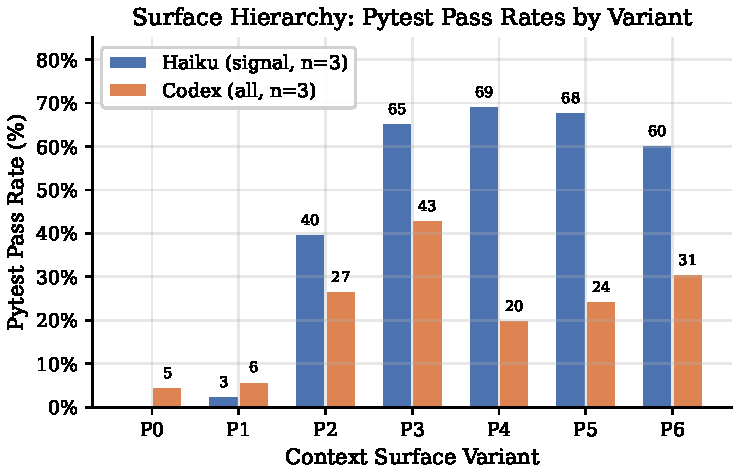
\includegraphics[width=\textwidth]{figures/fig1_surface_hierarchy.pdf}
\caption{Pytest pass rates by context surface variant for Haiku (26 signal bugs, $n{=}3$) and Codex (all 30 bugs, $n{=}3$, errors excluded). P4 (focused guide + autonomous retrieval) showed the highest mean rate for Haiku in these runs; Codex peaked at P3 (oracle injection). Note: Haiku and Codex are on different bug sets and are not directly comparable.}
\label{fig:surface-hierarchy}
\end{figure*}

\subsection{Causal Attribution}
\label{sec:causal-attribution}

To understand whether P4 performance is associated with VoltSnip retrieval rather than filesystem browsing or training-data pattern matching, four conditions were checked:

\begin{enumerate}
    \item \textbf{P0 = 0.0\%} on all 26 signal bugs --- the model cannot infer the org convention from training data alone. \checkmark
    \item \textbf{\texttt{voltsnip\_tool\_call\_count} $>$ 0} for passing P4 runs --- VoltSnip was actually called. \checkmark
    \item \textbf{\texttt{native\_tool\_call\_count} $=$ 0} for P4 runs --- no filesystem tools were available or used. \checkmark
    \item \textbf{P4 drops to $\approx$0\% when VoltSnip returns no snippets} --- tested via an ablation run with all snippets hidden (see below). \checkmark
\end{enumerate}

\textbf{Empty-store ablation.}
To close the attribution chain, one Haiku P4 evaluation ($n{=}1$, 26 signal bugs) was run with all VoltSnip snippets hidden via \texttt{is\_hidden=true} in the snippet store.
The model retained the SKILL.md guide and VoltSnip tools; tool calls succeeded but returned zero results.
The ablation pass rate was \textbf{0.0\%} (0/26) --- compared to 69.2\% for the standard P4 condition --- confirming that the SKILL.md guide framing alone, without retrievable snippet content, does not account for the observed lift.

Conditions 1--4 together support a retrieval-attribution interpretation: the lift from P0 to P4 comes from VoltSnip retrieval content, not from guide framing or filesystem browsing.

\begin{figure*}[t]
\centering
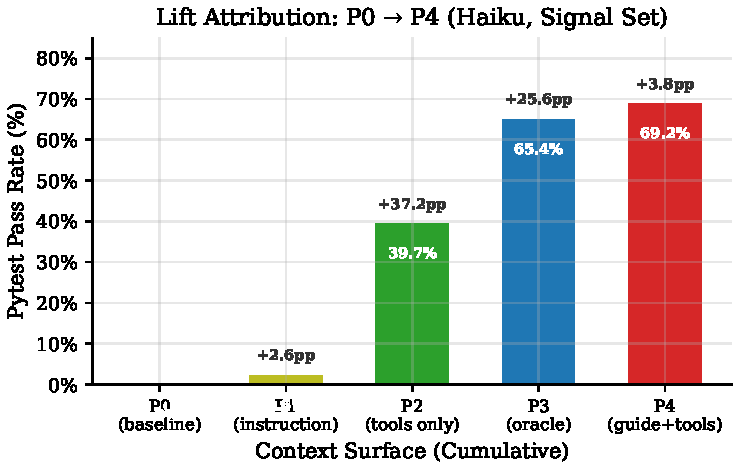
\includegraphics[width=\textwidth]{figures/fig3_lift_waterfall.pdf}
\caption{Cumulative lift from P0 (baseline) to P4 (highest-scoring variant) for Haiku on the 26-bug signal set. Each bar shows the absolute pass rate; annotations show incremental lift from the previous variant.}
\label{fig:lift-waterfall}
\end{figure*}

\subsection{Possible Over-Specification Effect (P6 $<$ P4)}
\label{sec:over-specification}

For Haiku, P6 (both guide documents + tools) scored 60.3\%, lower than P4 (SKILL.md only + tools) at 69.2\% --- an 8.9 percentage-point gap.
At $n{=}3$ with P4's inter-run range of 26.9~pp (Table~\ref{tab:per-run}), this gap is not statistically confirmed overall, but retrieval quality analysis points to a plausible mechanism.

Running \texttt{analyze\_retrieval\_quality.py} on the batch\_1 artefacts shows that P6 achieved \emph{full coverage} (both required snippets retrieved) in only 22.2\% of runs, compared to 36.1\% for P4.
More strikingly, when P6 \emph{did} retrieve both required snippets, it passed 100.0\% of the time (vs 92.3\% for P4 in the same condition).
This suggests the P6 deficit is a \emph{retrieval failure} --- having two guide documents appears to reduce the model's ability to issue effective search queries --- rather than a failure to apply retrieved knowledge once available.
This is consistent with findings that models under-utilise relevant information when context is long or competing~\citep{liu2023lostmiddle}, though here the mechanism appears to be degraded retrieval querying rather than failure to read available context.

\subsection{Cross-Model Divergence}
\label{sec:cross-model}

The surface hierarchy appears \textbf{not consistent} across model families, though the comparison is imperfect: Haiku results are on 26 signal bugs while Codex results are on all 30 bugs (including the 4 noisy bugs), and both have $n{=}3$ runs:

\begin{table*}[t]
\centering
\caption{Cross-model divergence on selected variants. Haiku: 26 signal bugs, $n{=}3$ runs. Codex: all 30 bugs, $n{=}3$ runs. The $\Delta$ column is approximate because the bug sets differ; direct comparison should be treated with caution.}
\label{tab:cross-model}
\begin{tabular}{@{}lcccc@{}}
\toprule
\textbf{Variant} & \textbf{Haiku} & \textbf{Codex} & $\boldsymbol{\Delta}$ \textbf{(H$-$C)} & \textbf{Bug set} \\
\midrule
P0                         & 0.0\%             & 4.7\%             & $-$4.7 pp  & $\approx$ \\
P3 (oracle)                & 65.4\%            & \textbf{43.0\%}   & $+$22.4 pp & $\approx$ \\
P4 (SKILL.md + tools)      & \textbf{69.2\%}   & 20.0\%            & $+$49.2 pp & $\approx$ \\
P5 (AGENTS.md + tools)     & 67.9\%            & 24.4\%            & $+$43.5 pp & $\approx$ \\
P6 (both + tools)          & 60.3\%            & 30.6\%            & $+$29.7 pp & $\approx$ \\
\bottomrule
\multicolumn{5}{l}{\small $\approx$ = not directly comparable (different bug sets).} \\
\end{tabular}
\end{table*}

\textbf{Observation}: Haiku showed P4 $>$ P3 in aggregate (though Run~1 reversed this: P3$=$61.5\% vs P4$=$57.7\%); Codex showed P3 $>$ P6 $>$ P5 $>$ P4 (static injection scored higher than dynamic retrieval).
For Codex, the highest-scoring variant (P3$=$43.0\%) uses no tools at all.

This divergence may reflect differences in tool-use proficiency between model families, but is hard to interpret given the different bug sets.
Codex P3 per-run values were: Run~1: 46.2\%, Run~2: 36.7\%, Run~3: 46.7\% --- relatively stable across runs (range 10~pp).
By contrast, Codex P4 showed much greater instability: Run~1: 46.2\%, Run~2: 6.7\%, Run~3: 10.0\% --- a 40~pp swing between Run~1 and Runs~2--3.
Run~3 (P4$=$10.0\%) is consistent with Run~2 rather than Run~1, which strengthens the observation that Codex struggles with VoltSnip tool-based retrieval in most runs.
Retrieval quality analysis (\texttt{analyze\_retrieval\_quality.py}) shows Codex P4 achieved full-coverage retrieval in only 3.6\% of runs across the first two Codex runs, compared to 36.1\% for Haiku P4; the third run is consistent with this pattern given its P4 pass rate of 10.0\%.
This near-zero retrieval recall in Codex P4 --- with two of three runs showing $\leq$10\% pass rates --- suggests that Codex was largely unable to issue effective VoltSnip queries in most runs, rather than reflecting a stable model preference for static injection.

\subsection{Per-Run Variance (Haiku)}
\label{sec:variance}

Haiku's three runs show moderate inter-run variance:

\begin{table*}[t]
\centering
\caption{Per-run pass rates for Haiku (26 signal bugs).}
\label{tab:per-run}
\begin{tabular}{@{}lccccr@{}}
\toprule
\textbf{Variant} & \textbf{Run 1} & \textbf{Run 2} & \textbf{Run 3} & \textbf{Mean} & \textbf{Range} \\
\midrule
P0 & 0.0\%  & 0.0\%  & 0.0\%  & 0.0\%  & 0 pp    \\
P2 & 30.8\% & 42.3\% & 46.2\% & 39.7\% & 15.4 pp \\
P3 & 61.5\% & 69.2\% & 65.4\% & 65.4\% & 7.7 pp  \\
P4 & 57.7\% & 84.6\% & 65.4\% & 69.2\% & 26.9 pp \\
P6 & 65.4\% & 61.5\% & 53.8\% & 60.3\% & 11.6 pp \\
\bottomrule
\end{tabular}
\end{table*}

P4 shows the widest range (26.9 pp), consistent with the stochastic nature of autonomous retrieval --- the model's retrieval strategy varies across runs.
P0 is perfectly stable at 0.0\% across all three runs, consistent with the zero-leakage design.

\begin{figure*}[t]
\centering
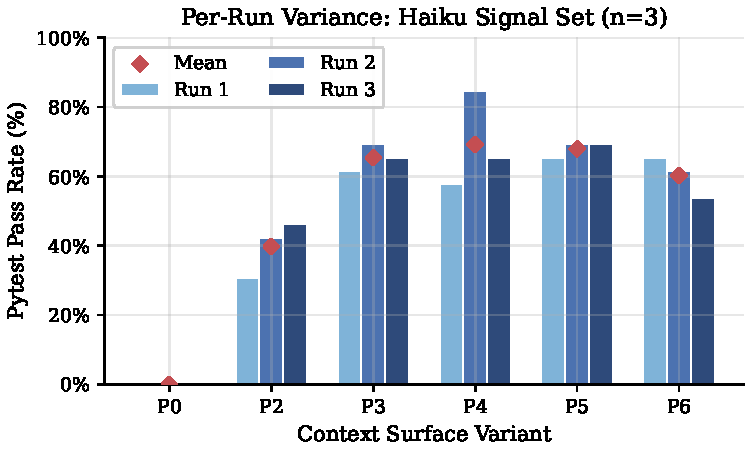
\includegraphics[width=\textwidth]{figures/fig2_per_run_variance.pdf}
\caption{Per-run pass rates for Haiku across three independent runs (26 signal bugs). P4 shows the widest inter-run variance (26.9~pp range), reflecting stochastic retrieval strategy. P0 is stable at 0.0\% across all runs.}
\label{fig:per-run-variance}
\end{figure*}

% ===================================================================
\section{Analysis and Discussion}
\label{sec:discussion}

\subsection{P4 vs P3: A Possible Retrieval-Cueing Effect}
\label{sec:p4-vs-p3}

P3 injects the exact correct snippets as fixed context, while P4 requires the model to retrieve them autonomously.
The aggregate result that P4 (69.2\%) $\geq$ P3 (65.4\%) for Haiku is interesting but not definitive: Run~1 showed P3 $>$ P4 (61.5\% vs 57.7\%), so the pattern does not hold in every run.

One speculative explanation is that the act of retrieval itself cues the model to attend to and apply the retrieved knowledge, rather than treating injected context as background that can be overlooked.
An alternative explanation is that P4's SKILL.md guide document provides additional value beyond retrieval cueing --- it frames \emph{how} to apply retrieved knowledge, not just \emph{what} to retrieve.
Retrieval quality analysis supports the second explanation: P4 passing runs ($N{=}54$) used a mean of 1.4 tool calls vs 0.7 for failing runs ($N{=}24$), and passing runs achieved full coverage (both required snippets retrieved) at a much higher rate.
P2 (tools, no guide) also shows a stark gap: when P2 retrieved both required snippets it passed 89.5\% of the time, but full coverage only occurred in 26.4\% of P2 runs vs 36.1\% for P4.
This suggests the SKILL.md guide raises retrieval success rate by directing the model to search more effectively, not just by providing framing context.

\subsection{Guide Document Effects}
\label{sec:guide-effects}

SKILL.md (P4) scored slightly higher than AGENTS.md (P5) for Haiku, and both scored higher than their combination (P6).
This is consistent with the idea that guide documents are useful for directing attention to retrieval, but stacking guides may introduce noise rather than signal.
This is consistent with SkillsBench's finding that focused Skills with 2--3 modules outperform comprehensive documentation~\citep{li2026skillsbench}, though the margins here are small and based on $n{=}3$ runs.

\subsection{Codex Divergence}
\label{sec:codex-divergence}

Codex's preference for static injection (P3) over dynamic retrieval (P4/P5) may reflect several factors:

\begin{enumerate}
    \item \textbf{Tool-use proficiency}: Codex may issue fewer or less effective VoltSnip search queries than Haiku.
    \item \textbf{MCP integration maturity}: The Codex HarnessMCPServer uses HTTP URL-based transport; protocol edge cases during the study required additional compliance work.
    \item \textbf{Inter-run variance}: Codex Runs~2 and~3 both showed low pass rates on tool-enabled variants (P4: 6.7\% and 10.0\% respectively, vs Run~1: 46.2\%), with Run~3 corroborating rather than explaining the Run~2 pattern. The persistence across two additional runs suggests this is not a transient infrastructure effect, but the mechanism remains unclear.
\end{enumerate}

\subsection{Tentative Implications for Practitioners}
\label{sec:implications}

If these pilot observations hold at larger $n$, the observed Haiku hierarchy (P4 $>$ P5 $>$ P3 $>$ P6 $>$ P2 $>$ P1 $\approx$ P0) would suggest:

\begin{itemize}
    \item \textbf{Retrieval tooling may matter more than prompt engineering.} The gap P4 $-$ P1 $=$ $+$66.6 pp for Haiku in these runs.
    \item \textbf{One focused guide document may be enough.} P4 scored higher than P6 by 8.9~pp, though this is not statistically confirmed.
    \item \textbf{Oracle injection may not be necessary}: autonomous retrieval (P4$=$69.2\%) scored comparably to oracle injection (P3$=$65.4\%), which matters because oracle injection requires upfront human curation of per-task relevant snippets --- expensive at scale.
    \item \textbf{For Codex-family models}: the data tentatively suggests static injection may work better than tool-based retrieval. With $n{=}3$ runs, P3 was stable (range 10~pp) while P4 was highly variable (range 40~pp, with two of three runs at $\leq$10\%), pointing to a tool-use issue rather than a model-level preference.
\end{itemize}

\subsection{Qualitative Failure Analysis}
\label{sec:qualitative}

Inspection of tool traces and model outputs across variants reveals four recurring failure modes:

\begin{enumerate}
    \item \textbf{Convention omission (P0--P1).} Without retrieval, models produce logically correct fixes but omit the \texttt{orgops.*} call entirely, or substitute a plausible-looking stub (e.g., \texttt{logging.info()} instead of \texttt{orgops.metrics.emit()}). The logic repair is present; only the org-policy component is missing. This is the dominant failure at P0 and P1.

    \item \textbf{Tool avoidance (P2, P6).} Even with tools available, models frequently skip tool calls and attempt a direct fix, especially without a guide document. Observed in P2 runs where the model produces a patch without issuing any VoltSnip query.

    \item \textbf{Poor query formulation (P2, P6).} When the model does call VoltSnip, overly broad queries (e.g., \texttt{"metrics"}) return snippets for unrelated bugs rather than the required ones. The full-coverage rate of 26.4\% for P2 vs 36.1\% for P4 reflects how SKILL.md improves query targeting. P6's two competing guides reduce effective query formulation further (22.2\% full-coverage rate).

    \item \textbf{Retrieved-but-misapplied (rare, $\sim$7.7\% of P4 full-coverage failures).} In a small number of runs where both required snippets were retrieved, the fix still failed pytest --- the model used an incorrect keyword argument name (e.g., \texttt{pct=} instead of \texttt{utilization\_pct=}) or applied the convention to the wrong call site. Retrieval recall is necessary but not sufficient.
\end{enumerate}

These four modes are consistent with the quantitative hierarchy: tool availability addresses omission failures; guide documents address tool avoidance and improve query quality; retrieval failure (modes 2--3, not misapplication) is the primary bottleneck at P2 and P6.

% ===================================================================
% ===================================================================
\section{Limitations}
\label{sec:limitations}

\begin{enumerate}
    \item \textbf{Benchmark construction.} Built by the author with full knowledge of bugs and required snippets; no third-party validation. Mitigations: bugs validated with P0$=$0 and P3$>$0 checks; four noisy bugs excluded with documented rationale; scoring uses Docker-isolated pytest. The benchmark tests \emph{composition execution}---fix a bug and apply a retrieved convention---not bug discovery. Logic errors are marked inline, so P0 failures reflect missing \texttt{orgops.*} calls, not failure to locate the bug.

    \item \textbf{Snippet fidelity.} Each scenario snippet provides the exact \texttt{orgops.*} call with prescribed arguments---near-complete specification of the fix. Real org knowledge bases are more abstract. This inflates absolute pass rates for P3--P6 relative to production, but does not affect the P3 vs P4 comparison (identical snippet content, delivery mechanism as the only variable).

    \item \textbf{Scoring precision.} Pytest checks exact \texttt{orgops.*} keyword argument names (e.g., \texttt{utilization\_pct=}, not \texttt{pct=}). A plausible but wrong name fails---by design, since the benchmark tests precise adherence to retrieved guidance, not approximate adherence.

    \item \textbf{Uniform difficulty labels.} All 30 tasks are labelled \texttt{difficulty: hard} with an uncalibrated \texttt{trap\_baseline} of 0.15, despite difficulty ranging from a single-character fix (BUG42) to recursive traversal with base64 decoding (BUG70). Snippet code fields are truncated to 1,200 characters; 12 snippets lose trailing content, but \texttt{orgops.*} details are preserved for all 12 and truncation is uniform across P3--P6.

    \item \textbf{Scale and corpus.} $n{=}3$ is small. Codex P4's 40~pp swing across runs illustrates per-variant sensitivity; Haiku's key observations (P0$=$0.0\%, P4 as top variant) held across all runs, though Run~1 showed P3 $>$ P4. The 35-snippet corpus likely understates real retrieval difficulty---corpus size is fixed across variants so relative comparisons remain valid.

    \item \textbf{Single codebase and language.} All 30 bugs are in one synthetic Python codebase. Generalisability to other languages (TypeScript, Java, Go) or real codebases is not established.

    \item \textbf{Residual provider asymmetry.}
    \label{sec:lim-asymmetry}
    Explicit shell/filesystem tools are disabled on both sides, but each provider retains a secondary read surface: Codex via sandbox background execution; Claude Code via \texttt{ReadMcpResourceTool}. The \texttt{cwd=tmpdir} boundary isolates both from \texttt{orgops/}; P0$=$0.0\% for both is consistent with isolation holding---but cross-provider comparisons carry this caveat.
\end{enumerate}

% ===================================================================
\section{Future Work}
\label{sec:future-work}

Several extensions would strengthen these observations:

\begin{enumerate}
    \item \textbf{More models.} Sonnet/Opus, GPT-5.2-Codex, and open-weight models would test whether the surface hierarchy generalises.
    \item \textbf{More Codex runs.} $n{=}5+$ with per-run tool traces would help distinguish infrastructure instability from a stable tool-use limitation.
    \item \textbf{Abstract snippets.} Rewriting snippets to give principle-level guidance rather than per-bug specs would test inference from abstract org knowledge---closer to production.
    \item \textbf{Larger corpus.} Scaling from 35 to 500+ snippets with distractors would stress-test retrieval robustness.
    \item \textbf{Difficulty tiers and negative controls.} Per-difficulty analysis and tasks with no applicable \texttt{orgops.*} convention would test over-application of retrieved patterns.
    \item \textbf{Other languages.} All 30 bugs are Python; TypeScript, Java, and Go would test cross-language generalisation.
    \item \textbf{Guide style ablation.} Minimal vs verbose, directive vs suggestive variants would further characterise the over-specification effect.
    \item \textbf{Hermetic isolation.} Docker-layer sandboxing for both providers would replace the current empirically-validated isolation with a hermetic guarantee.
    \item \textbf{Deeper retrieval traces.} Per-bug, per-run snippet utilisation traces would more cleanly separate ``never retrieved'' from ``retrieved but not applied'' failure modes.
\end{enumerate}

% ===================================================================
\section{Conclusion}
\label{sec:conclusion}

Script30 is a 30-bug composition benchmark where passing requires both a logic fix and a correct \texttt{orgops.*} call---a convention absent from training data. The seven-point P0--P6 ladder varies one delivery dimension at a time, enabling clean causal attribution of lift to specific context surfaces.

Key findings:

\begin{enumerate}
    \item \textbf{Zero leakage confirmed.} P0$=$0.0\% on signal bugs for both providers across all runs. The \texttt{orgops.*} API postdates both models' training data cutoffs.

    \item \textbf{Retrieval beats oracle injection (Haiku).} Autonomous retrieval with \texttt{SKILL.md} (P4$=$69.2\%) outperformed oracle injection (P3$=$65.4\%) in aggregate; an empty-store ablation (P4$=$0.0\%) confirmed the lift is retrieval-dependent, not a guide-framing effect.

    \item \textbf{Over-specification degrades retrieval (P6 $<$ P4).} Two guide documents reduced effective query formulation (22.2\% full-coverage rate vs 36.1\% for P4), though pass rate was 100\% when coverage was achieved---pointing to retrieval failure, not application failure.

    \item \textbf{Static injection more reliable for Codex.} P3 ($=$43.0\%) was stable across runs (range 10~pp); P4 was erratic (two of three runs $\leq$10\%, range 40~pp). Codex Run~1 also had 30 provider errors out of 210 cells, suggesting MCP tooling reliability issues independent of model capability.

    \item \textbf{Four failure modes identified.} Convention omission (P0--P1); tool avoidance (P2, P6); poor query formulation (P2, P6); retrieved-but-misapplied (rare, $\sim$7.7\% of P4 full-coverage failures). Retrieval failures (modes 2--3) are the dominant bottleneck.
\end{enumerate}

These are pilot findings at $n{=}3$, one Python codebase, two models. Generalisability to other languages, larger corpora, or different model families requires further study. The benchmark design and harness are reusable across models and retrieval backends. All code, run artefacts, and analysis scripts are at \url{https://github.com/vaddisrinivas/moltsnip} (branch \texttt{arxiv-v1}).


\section{Variant Ladder Formal Specification}
\label{app:variant-spec}

\begin{table*}[t]
\centering
\caption{Formal specification of the seven hypothesis variants.}
\label{tab:variant-spec}
\footnotesize
\begin{adjustbox}{max width=\textwidth}
\begin{tabular}{@{}llllllll@{}}
\toprule
\textbf{Field} & \textbf{P0} & \textbf{P1} & \textbf{P2} & \textbf{P3} & \textbf{P4} & \textbf{P5} & \textbf{P6} \\
\midrule
\texttt{mode}              & direct & direct & agent & agent & agent & agent & agent \\
\texttt{memory\_enabled}   & $\times$ & $\times$ & $\times$ & \checkmark & $\times$ & $\times$ & $\times$ \\
\texttt{tools\_enabled}    & $\times$ & $\times$ & \checkmark & $\times$ & \checkmark & \checkmark & \checkmark \\
\texttt{retrieval\_mode}   & none & none & agent\_dec. & injected & agent\_dec. & agent\_dec. & agent\_dec. \\
\texttt{instruction\_mode} & none & explicit & none & none & none & none & none \\
\texttt{context\_surface}  & user & user & tools\_only & system & skills\_md & agents\_md & both\_md \\
\texttt{max\_tool\_rtrips} & 1 & 1 & 4 & 4 & 4 & 4 & 4 \\
\bottomrule
\end{tabular}
\end{adjustbox}
\end{table*}

\section{All-Bugs Results (30 bugs, Haiku $n{=}3$)}
\label{app:all-bugs}

\begin{table}[t]
\centering
\caption{Pytest pass rates on all 30 bugs (Haiku, $n{=}3$).}
\label{tab:all-bugs}
\begin{tabular}{@{}lcr@{}}
\toprule
\textbf{Variant} & \textbf{Pass rate} & \textbf{Lift vs P0} \\
\midrule
P0 & 5.6\% (5/90)  & ---        \\
P1 & 6.7\% (6/90)  & $+$1.1 pp  \\
P2 & 42.2\% (38/90) & $+$36.6 pp \\
P3 & 65.6\% (59/90) & $+$60.0 pp \\
P4 & 71.1\% (64/90) & $+$65.5 pp \\
P5 & 71.1\% (64/90) & $+$65.5 pp \\
P6 & 61.1\% (55/90) & $+$55.5 pp \\
\bottomrule
\end{tabular}
\end{table}

\emph{Note: All-bugs results include the 4 noisy bugs (BUG41, BUG59, BUG62, BUG68) where P0 passes stochastically. The P0 rate of 5.6\% reflects passes on noisy bugs only. P4 and P5 are tied at 71.1\% in the all-bugs set despite P4 (69.2\%) $>$ P5 (67.9\%) on signal bugs; the noisy bugs slightly favour P5, erasing P4's signal-set advantage.}

\section{Harness Integrity Fixes Applied During Study}
\label{app:harness-fixes}

Three harness bugs were discovered and corrected during the study:

\begin{enumerate}
    \item \textbf{Stream error detection} (\texttt{claudecode.py}): Claude Code \texttt{is\_error=true} stream events were not propagated as provider errors, silently producing \texttt{status=ok} runs with empty code. Fixed by adding a stream error extractor.
    \item \textbf{Empty-output validity gate} (\texttt{runner.py}): runs with \texttt{status=ok} but no generated code were not demoted to error. Fixed by post-run validity check.
    \item \textbf{Resume integrity} (\texttt{csv\_mapper.py}): \texttt{load\_completed} loaded all entries regardless of status, preventing error runs from being retried on resume. Fixed by filtering to \texttt{status=ok}.
\end{enumerate}

All affected runs were re-executed after fixes were applied.

\section{Artefact Paths}
\label{app:artefacts}

All run artefacts (full model outputs, tool traces, scoring results, and pytest results) are available at:

\begin{center}
\url{https://github.com/vaddisrinivas/moltsnip}
\end{center}

\noindent Branch: \texttt{arxiv-v1}.
Run artefacts (CSV results, full model dumps, pytest logs, tool traces) are in the \texttt{vsevals\_runs/batch\_1/} subdirectory.

\begin{table*}[t]
\centering
\caption{Artefact locations in the repository (all paths relative to \texttt{vsevals/}).}
\label{tab:artefacts}
\footnotesize
\begin{tabular}{@{}lp{7cm}@{}}
\toprule
\textbf{Artefact} & \textbf{Path} \\
\midrule
Suite definition            & \texttt{suites/script30.yaml} \\
Task definitions (30 tasks) & \texttt{tasks/script30/BUG\{41..70\}.yaml} \\
Snippet corpus (35 snippets) & \texttt{snippets/script30/} \\
Usecase codebase            & \texttt{usecases/script30/} \\
Pytest tests (30 tests)     & \texttt{usecases/script30/tests/unit/test\_bug\{41..70\}.py} \\
Haiku Run 1                 & \texttt{.../batch\_1/matrix\_20260303T193221*} \\
Haiku Run 2                 & \texttt{.../batch\_1/matrix\_20260303T201709*} \\
Haiku Run 3                 & \texttt{.../batch\_1/matrix\_20260303T215606*} \\
Codex Run 1                 & \texttt{.../batch\_1/matrix\_20260303T193214*} \\
Codex Run 2                 & \texttt{.../batch\_1/matrix\_20260303T201241*} \\
Codex Run 3                 & \texttt{.../batch\_1/matrix\_20260304T083357*} \\
Ablation (empty-store)      & \texttt{.../batch\_1/matrix\_20260304T095907*} \\
Experiment log              & \texttt{EXPERIMENT.md} \\
Evaluation harness source   & \texttt{vsevals/} \\
Build script                & \texttt{scripts/build\_paper.py} \\
\bottomrule
\end{tabular}
\end{table*}

\subsection*{Claim-to-Evidence Mapping}

Every quantitative claim in this paper is mechanically derived from the CSV artefacts listed above via \texttt{scripts/build\_paper.py}.
The following table maps key claims to the run files and column fields that produce them.
Running \texttt{uv run python3 scripts/build\_paper.py --check} reproduces all numbers from the raw CSVs.

\begin{table*}[t]
\centering
\caption{Evidence mapping: paper claims to run artefacts and CSV fields.}
\label{tab:evidence}
\footnotesize
\begin{tabular}{@{}p{4cm}p{5.5cm}@{}}
\toprule
\textbf{Claim} & \textbf{Evidence source} \\
\midrule
P0 = 0.0\% on 26 signal bugs (Haiku) &
    Haiku Runs 1--3, \texttt{matrix\_results.csv}: filter \texttt{variant\_id=P0}, exclude noisy bugs, count \texttt{pytest\_passed=True} $\to$ 0/78. \\
P4 = 69.2\% (Haiku, 26 signal) &
    Haiku Runs 1--3, same CSV: filter \texttt{variant\_id=P4} $\to$ 54/78 passed. \\
P3 = 43.0\% (Codex, all 30 bugs) &
    Codex Runs 1--3, same CSV: filter \texttt{variant\_id=P3}, exclude \texttt{status$\neq$ok} $\to$ 37/86 passed. \\
Codex P4 = 20.0\% &
    Codex Runs 1--3: filter \texttt{variant\_id=P4}, exclude errors $\to$ 17/85. \\
P4 passing runs: 1.4 mean tool calls &
    Haiku Runs 1--3, CSV column \texttt{tool\_call\_count}: filter P4 signal, split by \texttt{pytest\_passed}. $N{=}54$ passing, $N{=}24$ failing. \\
P6 full-coverage = 22.2\% vs P4 = 36.1\% &
    \texttt{scripts/analyze\_retrieval\_quality.py} on batch\_1: column \texttt{required\_snippet\_coverage=1.0}. \\
Ablation P4 (empty store) &
    Ablation run CSV: filter \texttt{variant\_id=P4}, signal bugs only. \\
Run error counts (30/0/1) &
    Per-run: count rows where \texttt{pytest\_passed} is empty in each Codex run CSV. \\
\bottomrule
\end{tabular}
\end{table*}

% ===================================================================
\section{Metric Definitions: Pass Rate and Lift}
\label{app:metrics}

\textbf{Pass rate} is the fraction of scored runs in which Docker-isolated pytest exits with code~0.
For variant $v$ over bug set $B$ with $n$ valid runs:
\[
  \text{pass\_rate}(v) = \frac{\text{\# pytest-passed cells}}{\lvert B \rvert \times n}
\]
where cells with \texttt{status$\neq$ok} are excluded from both numerator and denominator.

\textbf{Lift} is the absolute percentage-point difference relative to P0:
\[
  \text{lift}(v) = \text{pass\_rate}(v) - \text{pass\_rate}(\text{P0})
\]
Lift is expressed in percentage points~(pp) and is \emph{not} a relative ratio.
A lift of $+$69.2~pp (Haiku P4) means P4 passes 69.2 percentage points more runs than P0, which itself passes 0.0\%.

% ===================================================================
\section{Model Inference Parameters and Training Data}
\label{app:model-details}

\subsection*{Inference configuration}

\begin{table}[h]
\centering
\caption{Per-provider inference configuration.}
\label{tab:inference-params}
\small
\begin{tabular}{@{}lll@{}}
\toprule
\textbf{Parameter} & \textbf{Haiku (Claude Code)} & \textbf{Codex (Codex CLI)} \\
\midrule
Model ID              & claude-haiku-4-5              & gpt-5.1-codex-mini \\
Temperature           & provider default              & provider default \\
Max tool roundtrips   & 4 (P2, P4--P6); 1 (P0--P3)   & 4 (P2, P4--P6); 1 (P0--P3) \\
Filesystem tools      & Blocked (\texttt{--disallowedTools}) & Blocked (\texttt{include\_fs\_tools=False}) \\
Shell access          & Blocked (Bash, Edit, Write)   & Read-only sandbox \\
Working directory     & Isolated tmpdir (per run)     & Isolated tmpdir (per run) \\
\bottomrule
\end{tabular}
\end{table}

Both providers were invoked with their CLI defaults; no explicit temperature override was applied.
Codex wipes globally-configured MCP servers for isolation; a residual read-only shell surface remains (see \S\ref{sec:lim-asymmetry}).

\subsection*{Training data and knowledge cutoff}

\textbf{claude-haiku-4-5}: training data cutoff approximately early 2025.
\textbf{gpt-5.1-codex-mini}: training data cutoff approximately early 2025.

The \texttt{orgops.*} API was constructed specifically for this benchmark, never published, and postdates both models' training cutoffs. Neither model was fine-tuned on the Script30 codebase or task descriptions. This is why both functions (\texttt{orgops.metrics.emit}, \texttt{orgops.audit.record}, etc.) cannot be inferred from training data, and why P0$=$0.0\% on signal bugs (Haiku, all three runs) serves as empirical confirmation of zero leakage.

\end{document}
